\chapter{Metode de analiză a imaginilor}\label{chapter:cap2}

Acest capitol prezintă principalele arhitecturi și concepte de deep learning relevante pentru problema studiată în lucrare. Este descrisă, în primul rând, structura generală a rețelelor neuronale convoluționale, alături de componentele lor fundamentale și de procesul de învățare prin care ponderile modelului sunt ajustate pe baza datelor de antrenare. Este prezentată în detaliu arhitectura AlexNet, utilizată ca model de bază în această lucrare, precum și principalele arhitecturi destinate segmentării imaginilor (U-Net, ResNet, EfficientNet), care oferă un context comparativ util pentru înțelegerea alegerilor metodologice din capitolele următoare. Capitolul se închide cu o prezentare a modelelor destinate identificării obiectelor din imagini, din familia YOLO, ale cărei principii sunt discutate în detaliu, prin raportare la lucrări existente, în Capitolul~\ref{chapter:cap3}.



\section{Rețele neuronale convoluționale}

Rețelele neuronale convoluționale (\textit{Convolutional Neural Networks}, CNN) reprezintă o clasă de arhitecturi de rețele neuronale specializate în procesarea datelor cu structură spațială, cum sunt imaginile. Conceptul a fost introdus de LeCun et al. \cite{lecun1998gradient}, care au demonstrat că învățarea automată a unor filtre convoluționale, aplicate local și partajate la nivelul întregii imagini, permite extragerea eficientă a trăsăturilor vizuale relevante pentru clasificare, reducând semnificativ numărul de parametri în comparație cu rețelele neuronale complet conectate. Arhitectura LeNet-5, una dintre primele rețele de acest tip, este ilustrată în Figura~\ref{fig:lenet5}.


\begin{figure}[H]
    \centering
    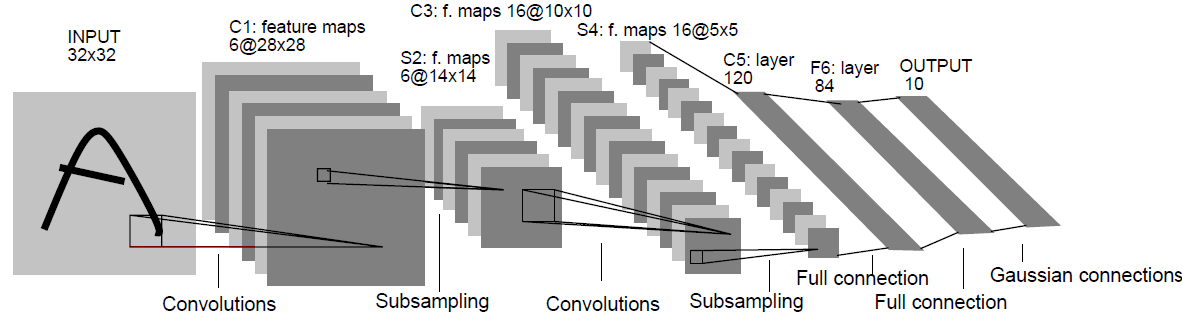
\includegraphics[width=0.85\textwidth]{figs/LeNet-5.png}
    \caption{Arhitectura LeNet-5, compusă din straturi convoluționale
    și de \textit{subsampling} alternante, urmate
    de straturi complet conectate \cite{lecun1998gradient}.}
    \label{fig:lenet5}
\end{figure}









\subsection{Componente fundamentale}

O rețea convoluțională este compusă, în mod tipic, dintr-o succesiune de blocuri convoluționale, urmate de unul sau mai multe straturi complet conectate care realizează clasificarea finală. Fiecare bloc convoluțional cuprinde, de regulă, mai multe tipuri de operații: convoluția propriu-zisă, normalizarea activărilor, funcția de activare neliniară și operația de agregare spațială (\textit{pooling}).

Stratul convoluțional aplică un set de filtre (\textit{kernels}) de dimensiuni reduse (de exemplu 3×3, 5×5 sau 11×11 pixeli) asupra imaginii de intrare, prin glisarea filtrului pe întreaga suprafață a imaginii și calcularea produsului scalar dintre ponderile filtrului și regiunea locală suprapusă la fiecare poziție. Fiecare filtru detectează un anumit tip de trăsătură vizuală: muchii, colțuri și texturi în straturile inferioare, forme și obiecte complexe în straturile superioare. Rezultatul aplicării unui filtru pe întreaga imagine formează o hartă de caracteristici (\textit{feature map}). Avantajul esențial al convoluției este partajarea ponderilor: același filtru este utilizat în toate pozițiile imaginii, ceea ce reduce drastic numărul de parametri ai modelului în comparație cu un strat complet conectat de aceeași dimensiune și introduce, în același timp, invarianța la translație.

Pe măsură ce rețelele convoluționale au devenit mai profunde, antrenarea lor a fost îngreunată de fenomenul \textit{internal covariate shift}: distribuția statistică a activărilor unui strat se modifică continuu pe parcursul antrenării, pe măsură ce ponderile straturilor anterioare sunt actualizate, ceea ce încetinește convergența și impune rate de învățare mai mici. O primă formă de normalizare a activărilor, introdusă chiar în arhitectura AlexNet \cite{krizhevsky2012imagenet}, este normalizarea locală a răspunsului (\textit{Local Response Normalization}, LRN), aplicată după funcția de activare ReLU în primele două straturi convoluționale și care reduce eroarea de clasificare cu 1.4 puncte procentuale pentru top-1 și 1.2 puncte procentuale pentru top-5 pe ILSVRC-2012. Câțiva ani mai târziu, normalizarea pe loturi (\textit{Batch Normalization}) \cite{ioffe2015batchnorm} a generalizat această idee, normalizând activările fiecărui strat la nivelul fiecărui mini-batch de antrenare, indiferent de poziția stratului în rețea, ceea ce permite utilizarea unor rate de învățare considerabil mai mari și o convergență mai rapidă. Datorită eficienței superioare, Batch Normalization a devenit standardul utilizat în arhitecturile convoluționale moderne, în locul LRN.

Ieșirea fiecărui strat convoluțional este trecută printr-o funcție de activare neliniară, cea mai utilizată în arhitecturile moderne fiind ReLU (\textit{Rectified Linear Unit}), definită ca $f(x) = \max(0, x)$ \cite{nair2010rectified}. Comparativ cu unitățile binare stocastice utilizate inițial în rețelele de tip Boltzmann, ReLU permite o reprezentare mai bogată a informației de intensitate și facilitează propagarea acesteia prin mai multe straturi de extragere a trăsăturilor \cite{nair2010rectified}.

După unul sau mai multe straturi convoluționale este frecvent aplicată o operație de pooling, care reduce dimensiunea spațială a hărților de caracteristici prin agregarea valorilor dintr-o vecinătate locală: de exemplu, {\it max-pooling} selectează valoarea maximă dintr-o fereastră de 2×2 sau 3×3 pixeli. Pooling-ul îndeplinește două roluri principale: reduce volumul de calcul necesar pentru straturile următoare și introduce un grad de invarianță la mici translații sau deformări ale obiectului din imagine.

O limitare importantă a rețelelor convoluționale foarte profunde este degradarea performanței la creșterea numărului de straturi, fenomen cauzat de dificultatea propagării gradientului prin multe straturi succesive. He et al. \cite{he2016resnet} au introdus conexiunile reziduale (\textit{skip connections}), prin care ieșirea unui bloc de straturi este adunată direct cu intrarea sa nemodificată, permițând gradientului să se propage mai facil înapoi prin rețea și făcând posibilă antrenarea unor arhitecturi cu sute de straturi.

După parcurgerea blocurilor convoluționale, reprezentarea extrasă este transmisă unor straturi complet conectate, similare celor dintr-o rețea neuronală clasică. Stratul final de ieșire este, în cazul problemelor de clasificare, activat printr-o funcție {\it softmax}, care transformă valorile brute de ieșire (\textit{logits}) într-o distribuție de probabilitate peste clasele posibile, astfel încât suma probabilităților asociate tuturor claselor să fie egală cu 1.


\subsection{Procesul de învățare}

Antrenarea unei rețele convoluționale constă în ajustarea iterativă a ponderilor modelului astfel încât predicțiile acestuia să se aproprie cât mai mult de etichetele reale ale datelor de antrenare. Acest proces necesită definirea unei funcții de pierdere (\textit{loss function}), care măsoară diferența dintre predicțiile modelului și etichetele corecte. Pentru probleme de clasificare, cea mai utilizată funcție de pierdere este entropia încrucișată (\textit{cross-entropy loss}), care penalizează cu atât mai mult o predicție cu cât probabilitatea atribuită clasei corecte este mai mică.

Minimizarea funcției de pierdere se realizează prin algoritmi de tip gradient descendent (\textit{gradient descent}), care actualizează ponderile modelului în direcția opusă gradientului funcției de pierdere în raport cu ponderile respective, calculat prin propagare inversă (\textit{backpropagation}). Algoritmul de bază, SGD (\textit{Stochastic Gradient Descent}), calculează gradientul pe subseturi mici de date (\textit{mini-batch-uri}) la fiecare pas de actualizare, în locul întregului set de antrenare, ceea ce reduce costul computațional și introduce un efect de regularizare prin natura sa stocastică. Implementările practice ale SGD includ frecvent un termen de momentum \cite{pytorch_sgd}, care acumulează o medie ponderată a gradienților anteriori pentru a stabiliza traiectoria de optimizare și a accelera convergența.

O alternativă larg utilizată este algoritmul Adam (\textit{Adaptive Moment Estimation}) \cite{kingma2014adam}, care adaptează rata de învățare individual pentru fiecare parametru al modelului, pe baza unor estimări ale primului și celui de-al doilea moment al gradienților. Adam converge frecvent mai rapid decât SGD clasic, în special pe seturi de date eterogene, dar poate fi mai predispus la suprapotrivire ({\it over-fitting}) pe seturi de date de dimensiuni reduse.

Performanța și comportamentul procesului de antrenare sunt influențate de o serie de hiperparametri (\textit{hyperparameters}), stabiliți înainte de antrenare și neactualizați prin procesul de propagare inversă. Dintre aceștia, cei mai importanți sunt rata de învățare (\textit{learning rate}), care controlează magnitudinea actualizărilor ponderilor la fiecare pas, și dimensiunea batch-ului (\textit{batch size}), care determină numărul de exemple utilizate pentru calcularea gradientului la o singură actualizare. O rată de învățare prea mare poate determina divergența procesului de optimizare, în timp ce o valoare prea mică poate conduce la o convergență excesiv de lentă sau la blocarea într-un minim local nesatisfăcător. Dimensiunea batch-ului influențează, de asemenea, calitatea estimării gradientului și capacitatea de generalizare a modelului rezultat, valori mai mici introducând un grad mai ridicat de zgomot stocastic, care poate favoriza, în anumite condiții, o generalizare mai bună.

Rata de învățare nu trebuie neapărat fixată pe întreaga durată a antrenării; ea poate fi ajustată dinamic printr-un planificator (\textit{scheduler}). O strategie frecvent utilizată în practică este reducerea ratei de învățare atunci când performanța modelului pe setul de validare stagnează pentru un număr fixat de epoci (\textit{ReduceLROnPlateau}) \cite{pytorch_reducelronplateau}, permițând o explorare inițială rapidă a spațiului de soluții, urmată de o rafinare mai precisă spre finalul antrenării.

Pentru a preveni supra-potrivirea (\textit{overfitting}), fenomen prin care modelul memorează particularitățile setului de antrenare în detrimentul capacității de generalizare, sunt utilizate frecvent tehnici de regularizare (\textit{regularization}). Dropout \cite{srivastava2014dropout} dezactivează aleatoriu o proporție din neuronii unui strat la fiecare pas de antrenare, forțând rețeaua să nu se bazeze excesiv pe combinații specifice de neuroni. O altă tehnică frecvent întâlnită este \textit{weight decay} \cite{krogh1991weightdecay}, care penalizează ponderile de magnitudine mare prin adăugarea unui termen proporțional cu norma acestora la funcția de pierdere, favorizând soluții mai simple și reducând riscul de supra-potrivire.  \textit{Label smoothing} \cite{szegedy2016labelsmoothing} este o tehnică similară, aplicată direct etichetelor de antrenare: în locul unei distribuții de probabilitate extreme (1 pentru clasa corectă, 0 pentru celelalte), se atribuie o probabilitate ușor redusă clasei corecte și o mică probabilitate reziduală celorlalte clase, reducând supra-încrederea modelului (\textit{overconfidence}) în predicțiile sale.



\section{Modele de clasificare a imaginilor}

\subsection{AlexNet}

În lucrarea \cite{krizhevsky2012imagenet}, Krizhevsky et al. prezintă arhitectura AlexNet, o rețea neuronală convoluțională profundă antrenată pe setul de date ImageNet LSVRC-2010, conținând 1.2 milioane de imagini distribuite în 1000 de clase. Lucrarea reprezintă un punct de referință în domeniul viziunii computerizate, demonstrând pentru prima dată că rețelele convoluționale profunde pot depăși semnificativ metodele clasice de extragere manuală a trăsăturilor pe seturi de date de mari dimensiuni.

Arhitectura propusă este compusă din cinci straturi convoluționale urmate de trei straturi complet conectate, ilustrate în Figura~\ref{fig:alexnet_cap2}. Primul strat convoluțional aplică 96 de filtre de dimensiune 11×11 cu pas 4 pe imaginile de intrare redimensionate la 224×224 pixeli. Straturile convoluționale ulterioare utilizează filtre de dimensiuni mai mici (5×5 și 3×3), cu operații de max-pooling intercalate pentru reducerea dimensiunii spațiale a hărților de caracteristici. Stratul de ieșire conține 1000 de neuroni, corespunzând celor 1000 de clase ImageNet, activați printr-o funcție softmax. Numărul total de parametri ai modelului depășește 60 de milioane.

\begin{figure}[H]
    \centering
    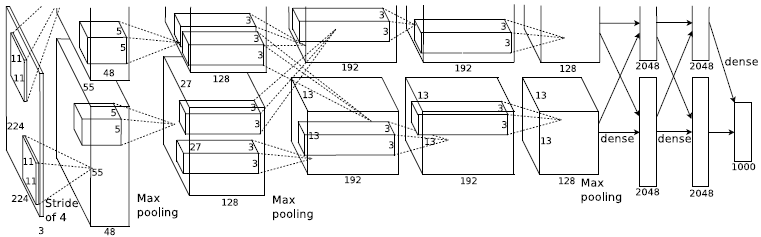
\includegraphics[width=\textwidth]{figs/AlexNetArhitectura.png}
    \caption{Arhitectura rețelei AlexNet cu cele cinci straturi
    convoluționale, operațiile de max-pooling și cele trei straturi
    complet conectate \cite{krizhevsky2012imagenet}.}
    \label{fig:alexnet_cap2}
\end{figure}

Lucrarea introduce mai multe contribuții tehnice care au devenit practici standard în deep learning. Funcția de activare ReLU (\textit{Rectified Linear Unit}) înlocuiește funcțiile sigmoidale clasice, accelerând convergența antrenării de câteva ori față de alternativele existente. Tehnica Dropout, aplicată cu o rată de 0.5 în straturile complet conectate, reduce supra-antrenarea prin dezactivarea aleatorie a neuronilor în timpul antrenării. Augmentarea datelor prin decupări și reflexii aleatorii ale imaginilor de antrenare contribuie suplimentar la regularizare. Antrenarea este realizată pe două unități GPU în paralel timp de cinci zile, utilizând metoda gradientului descendent stocastic cu moment.

Modelul a obținut o rată de eroare top-5 de 15.3\% pe setul de testare ILSVRC-2010, față de 26.2\% obținută de cel mai bun model alternativ din competiție, reprezentând o îmbunătățire de peste 10 puncte procentuale. Performanța a demonstrat că adâncimea rețelei este esențială: eliminarea oricăruia dintre straturile convoluționale intermediare conducea la degradarea semnificativă a acurateței.

Avantajele arhitecturii constau în capacitatea de a învăța automat reprezentări ierarhice ale trăsăturilor vizuale, de la muchii și texturi simple în straturile inferioare până la concepte semantice complexe în straturile superioare, fără a necesita inginerie manuală a trăsăturilor. Limitările includ numărul mare de parametri (peste 60 de milioane), care impune seturi de date mari pentru antrenare de la zero și resurse computaționale considerabile, precum și sensibilitatea la variațiile de iluminare și unghi în absența augmentării datelor.





\section{Modele pentru segmentarea imaginilor}

Segmentarea imaginilor reprezintă o categorie de sarcini de viziune computerizată
în care obiectivul este atribuirea unei etichete de clasă fiecărui pixel din imagine, spre diferență  de clasificare, unde se atribuie o singură etichetă întregii imagini, sau de detecția obiectelor, unde obiectele sunt localizate prin dreptunghiuri de încadrare. Rezultatul unei segmentări este o hartă de aceeași rezoluție cu imaginea de intrare, în care fiecare pixel este asociat clasei obiectului din care face parte, permițând o delimitare precisă a formei și conturului obiectelor de interes. Această granularitate ridicată face din segmentare o sarcină considerabil mai complexă din punct de vedere computațional decât clasificarea, dar și mult mai informativă pentru aplicații care necesită localizarea exactă a obiectelor, precum imagistica medicală sau analiza scenelor naturale.

\subsection{U-Net}

U-Net \cite{ronneberger2015unet} este una dintre cele mai influente arhitecturi dezvoltate pentru segmentare, propusă inițial pentru segmentarea imaginilor biomedicale.

Arhitectura U-Net este organizată simetric, sub forma literei U, fiind compusă din două componente principale: un {\it encoder} (calea de contractare), care extrage progresiv trăsături printr-o succesiune de straturi convoluționale și operații de pooling, reducând dimensiunea spațială a reprezentării, și un {\it decoder} (calea de expansiune), care reconstruiește dimensiunea spațială originală prin operații de up-sampling, generând în final o hartă de segmentare de aceeași rezoluție cu imaginea de intrare. Particularitatea esențială a U-Net constă în conexiunile directe (\textit{skip connections}) dintre straturile corespunzătoare ale encoder-ului și decoder-ului, prin care trăsăturile de detaliu spațial, pierdute parțial în procesul de contractare, sunt transmise direct către decoder, permițând o localizare mai precisă a obiectelor segmentate. O altă caracteristică notabilă a arhitecturii este capacitatea sa de a obține rezultate competitive folosind seturi de date de antrenare relativ mici, proprietate care a contribuit la adoptarea sa pe scară largă în domenii unde adnotarea pixel-cu-pixel este costisitoare, precum imagistica medicală. Structura arhitecturii este ilustrată în Figura~\ref{fig:unet}.

\begin{figure}[htbp]
    \centering
    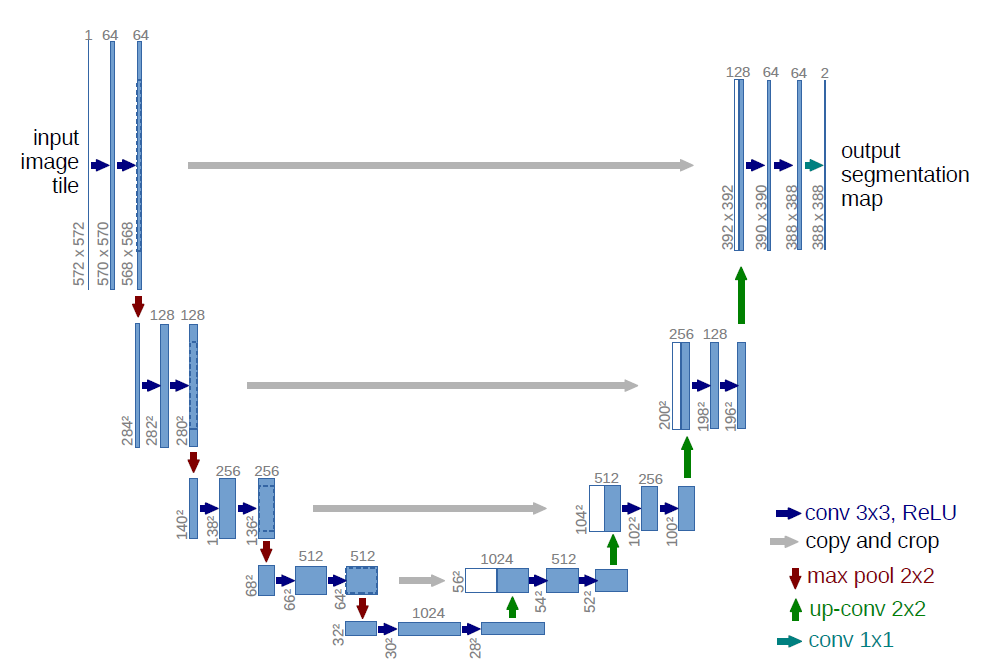
\includegraphics[width=\textwidth]{figs/UNetArhitectura.png}
    \caption{Arhitectura U-Net, ilustrând organizarea simetrică în
    formă de U a encoder-ului și decoder-ului \cite{ronneberger2015unet}.}
    \label{fig:unet}
\end{figure}

\subsection{ResNet}

Pe măsură ce rețelele convoluționale destinate clasificării au crescut în profunzime, cercetătorii au observat un fenomen de degradare a performanței: dincolo de un anumit număr de straturi, adăugarea de straturi suplimentare nu mai aducea o creștere a acurateței, ci, dimpotrivă, o deteriora, fenomen distinct de simpla suprapotrivire. Cauza principală este dificultatea propagării gradientului prin un număr mare de straturi succesive în procesul de propagare inversă. He et al. \cite{he2016resnet} au adresat această problemă prin introducerea arhitecturii ResNet (\textit{Residual Network}), bazată pe blocuri reziduale: în loc ca un bloc de straturi să învețe direct funcția de transformare dorită, acesta învață doar diferența (\textit{reziduul}) față de intrarea sa, care este adunată direct la ieșire printr-o conexiune reziduală. Această reformulare facilitează considerabil propagarea gradientului către straturile inferioare, permițând antrenarea unor rețele cu sute de straturi, comparativ cu câteva zeci de straturi posibile anterior. Cea mai profundă variantă propusă de autori, cu 152 de straturi, a obținut o eroare de doar 3,57\% pe setul de testare ImageNet, câștigând competiția ILSVRC din 2015. Structura blocului rezidual de bază este ilustrată în Figura~\ref{fig:resnet_block}, iar Figura~\ref{fig:resnet_arch} prezintă modul în care aceste blocuri sunt integrate într-o arhitectură completă, prin comparație cu o rețea convoluțională simplă de profunzime echivalentă.

\begin{figure}[htbp]
    \centering
    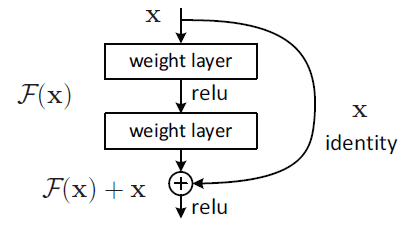
\includegraphics[width=0.5\textwidth]{figs/ResNetBlocRezidual.png}
    \caption{Blocul rezidual de bază propus de He et al.
    \cite{he2016resnet}.}
    \label{fig:resnet_block}
\end{figure}

\begin{figure}[htbp]
    \centering
    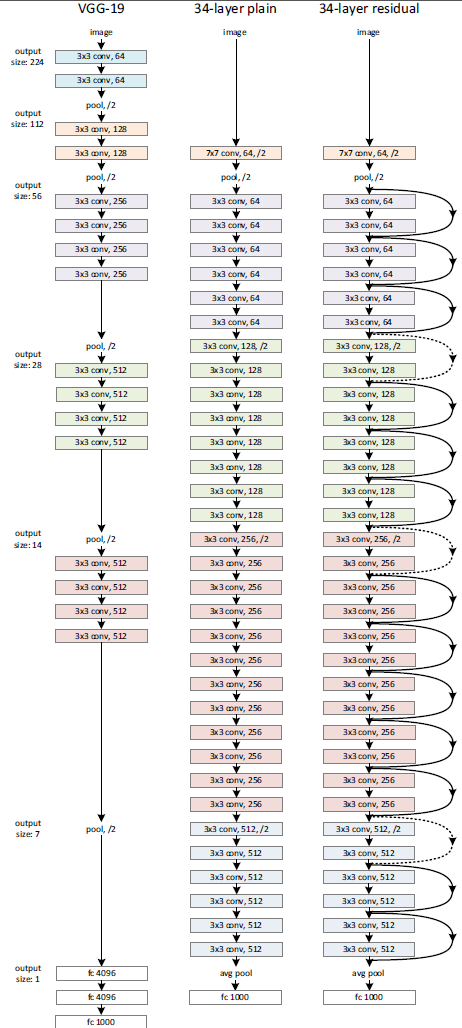
\includegraphics[height=0.85\textheight]{figs/ResNetArhitectura.png}
    \caption{Comparație între arhitectura VGG-19, o rețea
    convoluțională simplă cu 34 de straturi (\textit{34-layer plain})
    și varianta reziduală echivalentă (\textit{34-layer residual}),
    evidențiind conexiunile reziduale introduse la fiecare pereche
    de straturi \cite{he2016resnet}.}
    \label{fig:resnet_arch}
\end{figure}

\subsection{EfficientNet}

O direcție alternativă de dezvoltare a arhitecturilor convoluționale moderne s-a concentrat nu pe introducerea unor module noi, ci pe modul în care o arhitectură de bază este scalată pentru a obține performanțe superioare. Practica obișnuită înainte de  EfficientNet consta în scalarea arbitrară a unei singure dimensiuni a rețelei, fie prin creșterea profunzimii (numărul de straturi), fie a lățimii (numărul de filtre per strat), fie a rezoluției imaginilor de intrare. Tan și Le \cite{tan2019efficientnet} au demonstrat că o scalare echilibrată și simultană a tuturor celor trei dimensiuni, printr-un coeficient compus (\textit{compound scaling}) determinat printr-o căutare sistematică pe o arhitectură de bază, conduce la un raport considerabil mai favorabil între acuratețe și costul computațional decât scalarea independentă a unei singure dimensiuni. Familia de modele rezultată, EfficientNet, obține o acuratețe comparabilă sau superioară arhitecturilor anterioare, folosind un număr semnificativ mai redus de parametri, varianta cea mai performantă (EfficientNet-B7) atingând 84,3\% acuratețe top-1 pe ImageNet. Cele patru strategii de scalare, alături de scalarea compusă propusă, sunt ilustrate comparativ în Figura~\ref{fig:efficientnet}.

\begin{figure}[H]
    \centering
    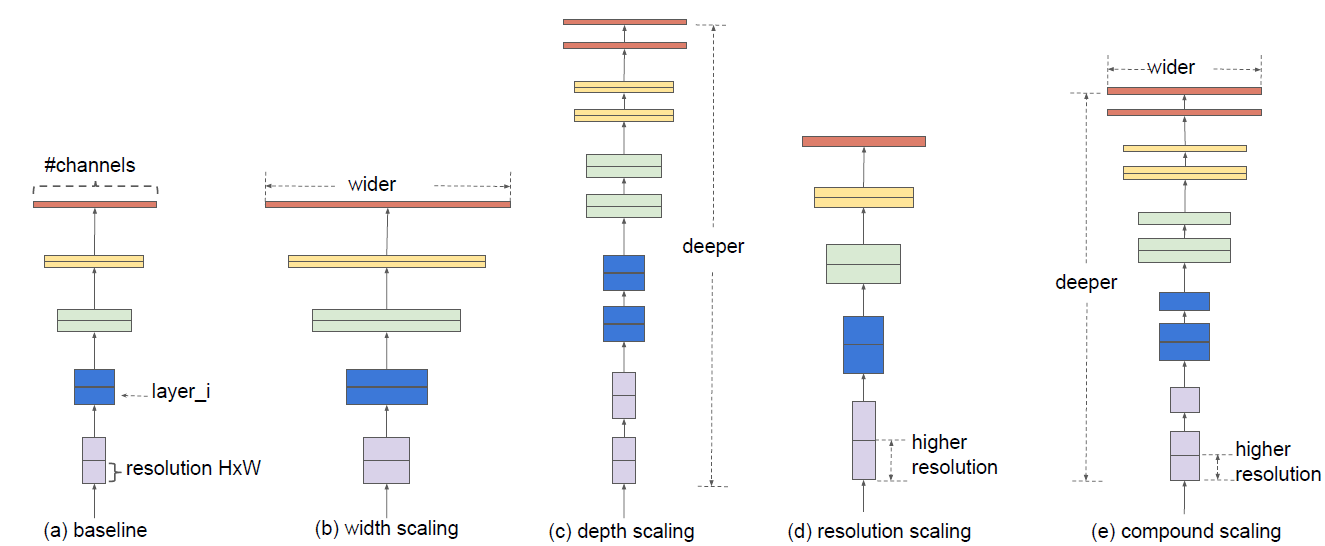
\includegraphics[width=\textwidth]{figs/EfficientNetScaling.png}
    \caption{Strategii de scalare a unei rețele convoluționale:
    referință (a), scalare în lățime (b), scalare în profunzime (c),
    scalare a rezoluției (d) și scalarea compusă (\textit{compound
    scaling}) propusă de EfficientNet (e) \cite{tan2019efficientnet}.}
    \label{fig:efficientnet}
\end{figure}







\section{Modele pentru identificarea obiectelor din imagini}

Detecția obiectelor este o sarcină intermediară între clasificare și segmentare: scopul nu este doar atribuirea unei etichete imaginii, ca în clasificare, dar nici delimitarea exactă a fiecărui pixel, ca în segmentare, ci localizarea obiectelor de interes prin dreptunghiuri de încadrare (\textit{bounding boxes}), însoțite de eticheta clasei corespunzătoare. Abordările anterioare anului 2016 tratau, în general, detecția în mai multe etape: o primă etapă propunea regiuni candidate din imagine, urmată de o etapă separată de clasificare a fiecărei regiuni propuse, ceea ce făcea procesul lent și dificil de optimizat de la un cap la altul.

YOLO (\textit{You Only Look Once}) \cite{redmon2016yolo} a schimbat fundamental această abordare, reformulând detecția ca o problemă unică de regresie. Imaginea de intrare este împărțită într-un grid de celule, iar pentru fiecare celulă o singură rețea convoluțională prezintă direct coordonatele dreptunghiurilor de încadrare și probabilitățile de clasă asociate, totul într-o singură trecere prin rețea. Această abordare unificată elimină nevoia unei etape separate de propunere a regiunilor candidate și permite optimizarea întregului proces de detecție direct pe performanța finală, aducând YOLO un avantaj considerabil de viteză: varianta originală a modelului prelucrează imagini la 45 de cadre pe secundă, suficient pentru detecție în timp real. Figura~\ref{fig:yolo_system} ilustrează fluxul general al sistemului de detecție, Figura~\ref{fig:yolo_model} detaliază modul în care gridul de celule generează dreptunghiurile de încadrare și harta probabilităților de clasă, iar Figura~\ref{fig:yolo_arch} prezintă arhitectura completă a rețelei convoluționale utilizate.

\begin{figure}[H]
    \centering
    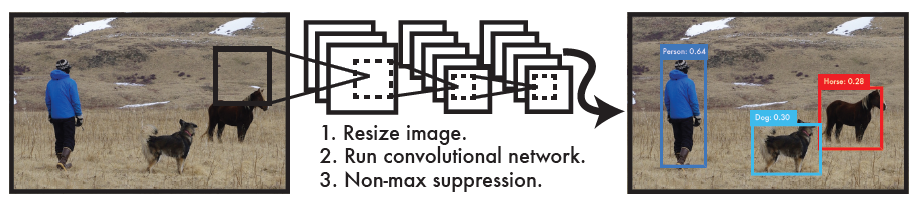
\includegraphics[width=\textwidth]{figs/YOLODetectionSystem.png}
    \caption{Sistemul de detecție YOLO: cei trei pași ai procesării,
    de la imaginea de intrare la detecțiile finale
    \cite{redmon2016yolo}.}
    \label{fig:yolo_system}
\end{figure}

\begin{figure}[H]
    \centering
    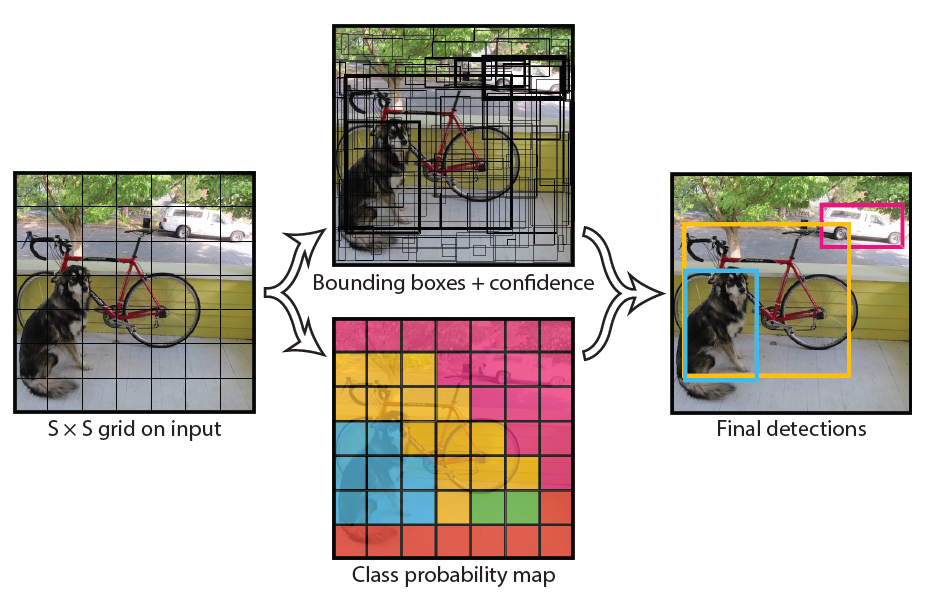
\includegraphics[width=0.75\textwidth]{figs/YOLOModel.png}
    \caption{Modelul YOLO: imaginea este împărțită într-un grid
    $S \times S$, pentru fiecare celulă fiind prezise dreptunghiuri
    de încadrare cu scoruri de încredere asociate și o hartă a
    probabilităților de clasă, combinate în detecțiile finale
    \cite{redmon2016yolo}.}
    \label{fig:yolo_model}
\end{figure}

\begin{figure}[H]
    \centering
    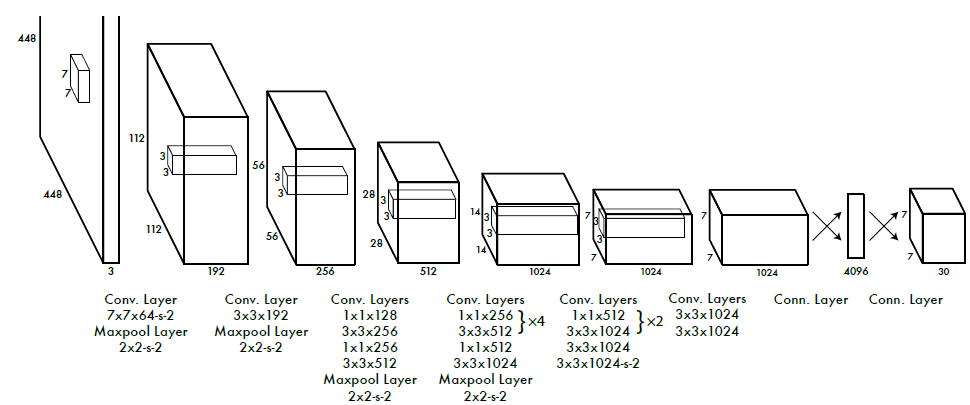
\includegraphics[width=\textwidth]{figs/YOLOArhitectura.png}
    \caption{Arhitectura rețelei YOLO, compusă din 24 de straturi
    convoluționale urmate de 2 straturi complet conectate. Straturile
    de reducere $1\times1$, alternate cu straturi convoluționale
    $3\times3$, reduc numărul de canale înainte de procesarea spațială
    ulterioară \cite{redmon2016yolo}.}
    \label{fig:yolo_arch}
\end{figure}

De la publicarea variantei inițiale, arhitectura YOLO a fost extinsă și rafinată în numeroase versiuni succesive, fiecare aducând îmbunătățiri la nivelul vitezei, acurateței sau dimensiunii modelului. Capitolul \ref{chapter:cap3} discută în detaliu două astfel de versiuni, YOLOv11n și YOLOv8n, aplicate specific pe sarcina detecției și segmentării specimenelor de raci de apă dulce, ilustrând modul în care principiul de bază introdus de YOLO a fost adaptat pentru aplicații practice de monitorizare a biodiversității acvatice.












% arhitectura
% nuclee de convoluție (kernels), module de agregare și redimensionare (pooling), nivel de clasificare (softmax)
% proces de învățare:  funcție de eroare, algoritmi de antrenare (SGD, ADAM, etc), hiperparametri (batch size, learning rate etc)
%\section{Modele pentru segmentarea imaginilor}
% UNet
% ResNet
% EfficientNet
%\section{Modele pentru identificarea obiectelor din imagini}
% YOLO